% !TeX root = ../main.tex
% !TeX encoding = UTF-8
% !TeX spellcheck = none
\subsection{主要实验结果}\label{sec:exp-main-results}

本节从总体预测精度、空间分布、常规模式偏离情景及残差作用四个方面评价CMSRN，结合全测试集比较与固定模型诊断，考察两类修正证据在不同交通状态下的表现。

\subsubsection{整体预测性能}\label{sec:results-overall}

表~\ref{tab:chengdu-inflow}--\ref{tab:shanghai-outflow}比较了CMSRN与13种基线在成都和上海流入、流出预测任务上的表现。在上述13种基线的比较范围内，CMSRN在32个表列指标中取得26项最优，其余6项均排名第二；在反映整个预测区间表现的8项AVG12指标中，取得7项最优。以下相对变化均根据未舍入数值计算，并以对应任务和指标的最强基线为参照。

CMSRN在两个城市的流入与流出任务上均取得最低AVG12 MAE。成都流入和流出的AVG12 MAE分别为0.708和0.709，相较于HyperD分别降低2.00\%和0.46\%；上海流入和流出的对应结果为0.728和0.774，分别降低1.19\%和0.46\%。

RMSE呈现出更明显的任务差异。成都流入、成都流出和上海流入的AVG12 RMSE分别为1.294、1.223和1.228，相较于各自最强基线分别降低5.01\%、1.50\%和2.54\%；前两项的最强基线为STGCN，后一项为HyperD。上海流出的AVG12 RMSE为1.346，略高于HyperD的1.344，相对差距为0.17\%。因此，CMSRN在流入预测上的双指标优势更为一致，在流出预测上则与最强基线较为接近。

从预测时距看，CMSRN在两个城市的流入任务上均取得H3、H6和H12的最低MAE与RMSE。随着时距由H3延伸至H12，CMSRN在四个任务上的MAE增幅为0.73\%--1.85\%，RMSE增幅为0.53\%--2.83\%。流出任务的优势则未覆盖所有时距和指标：两个城市在H12的MAE均由HyperD取得最优，在上海流出任务上，HyperD在三个报告时距的RMSE也均略低于CMSRN。

% !TeX root = ../main.tex
% !TeX spellcheck = none
\begin{table}[!htbp]
\centering
\caption{成都流入预测结果（\(32\times32\)网格）}
\label{tab:chengdu-inflow}
\begingroup
\linespread{1}\fontsize{10}{12}\selectfont
\setlength{\tabcolsep}{4.5pt}
\renewcommand{\arraystretch}{1.05}
\begin{tabular*}{\linewidth}{@{\extracolsep{\fill}}l*{8}{r}@{}}
\toprule
& \multicolumn{2}{c}{H3} & \multicolumn{2}{c}{H6} & \multicolumn{2}{c}{H12} & \multicolumn{2}{c}{AVG12} \\
\cmidrule(l{4.5pt}r{4.5pt}){2-3}\cmidrule(l{4.5pt}r{4.5pt}){4-5}\cmidrule(l{4.5pt}r{4.5pt}){6-7}\cmidrule(l{4.5pt}r{4.5pt}){8-9}
模型 & MAE & RMSE & MAE & RMSE & MAE & RMSE & MAE & RMSE \\
\midrule
HA & 1.053 & 1.522 & 1.083 & 1.600 & 1.144 & 1.739 & 1.088 & 1.609 \\
SVR & 0.810 & 1.354 & 0.835 & 1.391 & 0.892 & 1.499 & 0.840 & 1.405 \\
DCRNN (ICLR'18) & 0.725 & \underline{1.321} & 0.790 & 1.363 & 1.025 & 1.574 & 0.829 & 1.399 \\
STGCN (IJCAI'18) & 0.721 & 1.342 & 0.724 & \underline{1.348} & 0.743 & 1.409 & 0.728 & \underline{1.362} \\
GWNet (IJCAI'19) & \underline{0.719} & 1.332 & 0.731 & 1.373 & 0.756 & 1.450 & 0.733 & 1.378 \\
DSTAGNN (ICML'22) & 1.022 & 1.461 & 1.008 & 1.458 & 1.044 & 1.505 & 1.027 & 1.473 \\
PDFormer (AAAI'23) & 1.703 & 2.728 & 1.704 & 2.728 & 1.703 & 2.727 & 1.704 & 2.727 \\
PatchTST (ICLR'23) & 0.799 & 1.405 & 0.826 & 1.483 & 0.880 & 1.614 & 0.831 & 1.490 \\
TimeMixer (ICLR'24) & 0.818 & 1.434 & 0.844 & 1.505 & 0.895 & 1.620 & 0.848 & 1.510 \\
STDN (AAAI'25) & 1.178 & 1.589 & 1.180 & 1.593 & 1.179 & 1.600 & 1.178 & 1.593 \\
MetaDG (AAAI'26) & 1.102 & 1.564 & 1.170 & 1.678 & 1.291 & 1.882 & 1.178 & 1.692 \\
HyperD (AAAI'26) & 0.723 & 1.369 & \underline{0.723} & 1.369 & \underline{0.726} & \underline{1.382} & \underline{0.723} & 1.369 \\
RAST (AAAI'26) & 0.724 & 1.332 & 0.734 & 1.372 & 0.756 & 1.446 & 0.736 & 1.377 \\
\midrule
\textbf{CMSRN (Ours)} & \textbf{0.704} & \textbf{1.282} & \textbf{0.707} & \textbf{1.290} & \textbf{0.717} & \textbf{1.318} & \textbf{0.708} & \textbf{1.294} \\
\bottomrule
\end{tabular*}
\endgroup
\par\smallskip
\begin{minipage}{\linewidth}
\footnotesize\linespread{1.1}\selectfont\raggedright
注：粗体与下划线分别表示最优和次优结果。H3、H6和H12对应15、30和60分钟预测，AVG12为全部12个单步指标的算术平均。排名依据未舍入数值确定，显示值相同不代表并列。
\end{minipage}
\end{table}

% !TeX root = ../main.tex
% !TeX spellcheck = none
\begin{table}[!htbp]
\centering
\caption{成都流出预测结果（\(32\times32\)网格）}
\label{tab:chengdu-outflow}
\begingroup
\linespread{1}\fontsize{10}{12}\selectfont
\setlength{\tabcolsep}{4.5pt}
\renewcommand{\arraystretch}{1.05}
\begin{tabular*}{\linewidth}{@{\extracolsep{\fill}}l*{8}{r}@{}}
\toprule
& \multicolumn{2}{c}{H3} & \multicolumn{2}{c}{H6} & \multicolumn{2}{c}{H12} & \multicolumn{2}{c}{AVG12} \\
\cmidrule(l{4.5pt}r{4.5pt}){2-3}\cmidrule(l{4.5pt}r{4.5pt}){4-5}\cmidrule(l{4.5pt}r{4.5pt}){6-7}\cmidrule(l{4.5pt}r{4.5pt}){8-9}
模型 & MAE & RMSE & MAE & RMSE & MAE & RMSE & MAE & RMSE \\
\midrule
HA & 1.023 & 1.404 & 1.043 & 1.439 & 1.085 & 1.510 & 1.047 & 1.445 \\
SVR & 0.792 & 1.239 & 0.809 & 1.251 & 0.838 & 1.285 & 0.810 & 1.255 \\
DCRNN (ICLR'18) & 0.714 & \underline{1.230} & 0.761 & \underline{1.237} & 1.151 & 1.642 & 0.844 & 1.326 \\
STGCN (IJCAI'18) & 0.714 & 1.235 & 0.716 & 1.239 & 0.725 & 1.258 & 0.718 & \underline{1.242} \\
GWNet (IJCAI'19) & 0.713 & 1.253 & 0.718 & 1.265 & 0.729 & 1.289 & 0.719 & 1.267 \\
DSTAGNN (ICML'22) & 1.018 & 1.383 & 1.007 & 1.376 & 1.035 & 1.410 & 1.021 & 1.390 \\
PDFormer (AAAI'23) & 1.601 & 2.375 & 1.601 & 2.375 & 1.602 & 2.376 & 1.601 & 2.375 \\
PatchTST (ICLR'23) & 0.786 & 1.300 & 0.802 & 1.333 & 0.837 & 1.396 & 0.805 & 1.337 \\
TimeMixer (ICLR'24) & 0.807 & 1.315 & 0.823 & 1.345 & 0.856 & 1.404 & 0.826 & 1.349 \\
STDN (AAAI'25) & 1.135 & 1.501 & 1.135 & 1.501 & 1.135 & 1.503 & 1.134 & 1.500 \\
MetaDG (AAAI'26) & 1.082 & 1.471 & 1.139 & 1.543 & 1.245 & 1.672 & 1.146 & 1.550 \\
HyperD (AAAI'26) & \underline{0.712} & 1.249 & \underline{0.712} & 1.249 & \textbf{0.714} & \underline{1.254} & \underline{0.712} & 1.249 \\
RAST (AAAI'26) & 0.718 & 1.242 & 0.724 & 1.257 & 0.735 & 1.282 & 0.724 & 1.258 \\
\midrule
\textbf{CMSRN (Ours)} & \textbf{0.706} & \textbf{1.220} & \textbf{0.708} & \textbf{1.222} & \underline{0.715} & \textbf{1.234} & \textbf{0.709} & \textbf{1.223} \\
\bottomrule
\end{tabular*}
\endgroup
\par\smallskip
\begin{minipage}{\linewidth}
\footnotesize\linespread{1.1}\selectfont\raggedright
注：粗体与下划线分别表示最优和次优结果。H3、H6和H12对应15、30和60分钟预测，AVG12为全部12个单步指标的算术平均。排名依据未舍入数值确定，显示值相同不代表并列。
\end{minipage}
\end{table}

% !TeX root = ../main.tex
% !TeX spellcheck = none
\begin{table}[!htbp]
\centering
\caption{上海流入预测结果（\(32\times32\)网格）}
\label{tab:shanghai-inflow}
\begingroup
\linespread{1}\fontsize{10}{12}\selectfont
\setlength{\tabcolsep}{4.5pt}
\renewcommand{\arraystretch}{1.05}
\begin{tabular*}{\linewidth}{@{\extracolsep{\fill}}l*{8}{r}@{}}
\toprule
& \multicolumn{2}{c}{H3} & \multicolumn{2}{c}{H6} & \multicolumn{2}{c}{H12} & \multicolumn{2}{c}{AVG12} \\
\cmidrule(l{4.5pt}r{4.5pt}){2-3}\cmidrule(l{4.5pt}r{4.5pt}){4-5}\cmidrule(l{4.5pt}r{4.5pt}){6-7}\cmidrule(l{4.5pt}r{4.5pt}){8-9}
模型 & MAE & RMSE & MAE & RMSE & MAE & RMSE & MAE & RMSE \\
\midrule
HA & 1.019 & 1.437 & 1.040 & 1.490 & 1.080 & 1.593 & 1.043 & 1.498 \\
SVR & 0.817 & 1.251 & 0.837 & 1.274 & 0.879 & 1.344 & 0.841 & 1.283 \\
DCRNN (ICLR'18) & \underline{0.734} & \underline{1.243} & 0.748 & 1.262 & 0.808 & 1.328 & 0.758 & 1.272 \\
STGCN (IJCAI'18) & 0.741 & 1.257 & 0.743 & 1.260 & 0.754 & 1.293 & 0.745 & 1.268 \\
GWNet (IJCAI'19) & 0.735 & 1.268 & 0.742 & 1.288 & 0.760 & 1.343 & 0.744 & 1.295 \\
DSTAGNN (ICML'22) & 1.010 & 1.410 & 0.950 & 1.360 & 1.009 & 1.426 & 0.994 & 1.402 \\
PDFormer (AAAI'23) & 1.592 & 2.472 & 1.591 & 2.471 & 1.589 & 2.468 & 1.591 & 2.471 \\
PatchTST (ICLR'23) & 0.800 & 1.333 & 0.816 & 1.382 & 0.849 & 1.480 & 0.819 & 1.392 \\
TimeMixer (ICLR'24) & 0.821 & 1.331 & 0.836 & 1.372 & 0.868 & 1.463 & 0.839 & 1.381 \\
STDN (AAAI'25) & 1.219 & 1.651 & 1.220 & 1.659 & 1.219 & 1.683 & 1.218 & 1.661 \\
MetaDG (AAAI'26) & 1.082 & 1.517 & 1.168 & 1.624 & 1.421 & 1.944 & 1.201 & 1.667 \\
HyperD (AAAI'26) & 0.737 & 1.261 & \underline{0.737} & 1.261 & \underline{0.737} & \underline{1.263} & \underline{0.737} & \underline{1.260} \\
RAST (AAAI'26) & 0.736 & 1.245 & 0.740 & \underline{1.259} & 0.749 & 1.289 & 0.741 & 1.261 \\
\midrule
\textbf{CMSRN (Ours)} & \textbf{0.726} & \textbf{1.221} & \textbf{0.727} & \textbf{1.225} & \textbf{0.734} & \textbf{1.241} & \textbf{0.728} & \textbf{1.228} \\
\bottomrule
\end{tabular*}
\endgroup
\par\smallskip
\begin{minipage}{\linewidth}
\footnotesize\linespread{1.1}\selectfont\raggedright
注：粗体与下划线分别表示最优和次优结果。H3、H6和H12对应15、30和60分钟预测，AVG12为全部12个单步指标的算术平均。排名依据未舍入数值确定，显示值相同不代表并列。
\end{minipage}
\end{table}

% !TeX root = ../main.tex
% !TeX spellcheck = none
\begin{table}[!htbp]
\centering
\caption{上海流出预测结果（\(32\times32\)网格）}
\label{tab:shanghai-outflow}
\begingroup
\linespread{1}\fontsize{10}{12}\selectfont
\setlength{\tabcolsep}{4.5pt}
\renewcommand{\arraystretch}{1.05}
\begin{tabular*}{\linewidth}{@{\extracolsep{\fill}}l*{8}{r}@{}}
\toprule
& \multicolumn{2}{c}{H3} & \multicolumn{2}{c}{H6} & \multicolumn{2}{c}{H12} & \multicolumn{2}{c}{AVG12} \\
\cmidrule(l{4.5pt}r{4.5pt}){2-3}\cmidrule(l{4.5pt}r{4.5pt}){4-5}\cmidrule(l{4.5pt}r{4.5pt}){6-7}\cmidrule(l{4.5pt}r{4.5pt}){8-9}
模型 & MAE & RMSE & MAE & RMSE & MAE & RMSE & MAE & RMSE \\
\midrule
HA & 1.059 & 1.528 & 1.079 & 1.559 & 1.118 & 1.629 & 1.082 & 1.565 \\
SVR & 0.866 & 1.373 & 0.882 & 1.395 & 0.914 & 1.447 & 0.883 & 1.398 \\
DCRNN (ICLR'18) & 0.782 & 1.355 & 0.794 & 1.365 & 0.856 & 1.388 & 0.804 & 1.365 \\
STGCN (IJCAI'18) & 0.784 & 1.353 & 0.787 & 1.359 & 0.797 & 1.385 & 0.789 & 1.364 \\
GWNet (IJCAI'19) & 0.783 & 1.381 & 0.788 & 1.394 & 0.801 & 1.424 & 0.789 & 1.396 \\
DSTAGNN (ICML'22) & 1.017 & 1.462 & 0.994 & 1.446 & 1.080 & 1.535 & 1.016 & 1.469 \\
PDFormer (AAAI'23) & 1.720 & 2.726 & 1.720 & 2.726 & 1.719 & 2.724 & 1.720 & 2.726 \\
PatchTST (ICLR'23) & 0.848 & 1.439 & 0.863 & 1.465 & 0.897 & 1.533 & 0.866 & 1.473 \\
TimeMixer (ICLR'24) & 0.869 & 1.448 & 0.883 & 1.473 & 0.915 & 1.538 & 0.886 & 1.480 \\
STDN (AAAI'25) & 1.109 & 1.591 & 1.107 & 1.593 & 1.105 & 1.605 & 1.106 & 1.595 \\
MetaDG (AAAI'26) & 1.127 & 1.600 & 1.245 & 1.748 & 1.599 & 2.238 & 1.298 & 1.825 \\
HyperD (AAAI'26) & \underline{0.778} & \textbf{1.344} & \underline{0.778} & \textbf{1.344} & \textbf{0.778} & \textbf{1.347} & \underline{0.778} & \textbf{1.344} \\
RAST (AAAI'26) & 0.787 & 1.366 & 0.792 & 1.380 & 0.804 & 1.409 & 0.793 & 1.381 \\
\midrule
\textbf{CMSRN (Ours)} & \textbf{0.773} & \underline{1.346} & \textbf{0.774} & \underline{1.345} & \underline{0.778} & \underline{1.353} & \textbf{0.774} & \underline{1.346} \\
\bottomrule
\end{tabular*}
\endgroup
\par\smallskip
\begin{minipage}{\linewidth}
\footnotesize\linespread{1.1}\selectfont\raggedright
注：粗体与下划线分别表示最优和次优结果。H3、H6和H12对应15、30和60分钟预测，AVG12为全部12个单步指标的算术平均。排名依据未舍入数值确定，显示值相同不代表并列。
\end{minipage}
\end{table}


\subsubsection{空间预测表现}\label{sec:results-spatial}

空间案例与后续情景分析保留生成图件时的预测输出；成都整体性能比较采用本次更新结果。图~\ref{fig:cmsrn-spatial-h6}进一步展示两个城市在H6的空间预测案例。CMSRN保留了主要高流量区域的空间位置，能够反映流量集中分布的结构；与此同时，部分热点的峰值强度和低流量区域仍存在幅值偏差。该空间对照补充展示了模型对区域流量分布的刻画能力及局部误差特征。

\begin{figure}[!htbp]
  \centering
  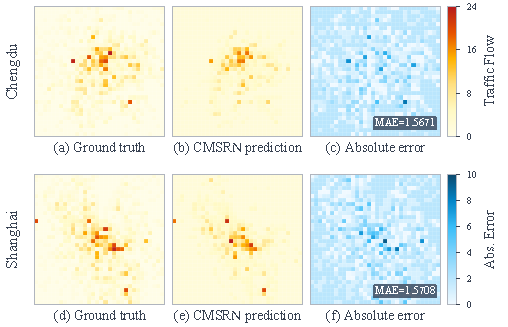
\includegraphics[width=\linewidth]{figures/cmsrn-spatial-h6.pdf}
  \caption[H6空间预测案例]{\textbf{第6个预测步（提前30分钟）的空间预测案例。}上排（a）--（c）为成都2016年11月25日09:50，下排（d）--（f）为上海2016年8月25日20:20，依次展示真实流量、CMSRN预测和绝对误差。每幅图表示原始\(32\times32\)网格上单个5分钟时间片的流入量与流出量之和；两城市采用统一色标，右侧上、下色条分别对应总流量与绝对误差。图内MAE为该时间片总流量在全部1,024个网格上的平均绝对误差，表格指标则按流量通道在测试集的正目标位置上计算。案例依据误差与空间对比度事后选取，时间均为UTC+8。}
  \label{fig:cmsrn-spatial-h6}
\end{figure}

% 情景性能与两条残差通路的分析统一纳入5.2。
% !TeX root = ../main.tex
% !TeX encoding = UTF-8
% !TeX spellcheck = none
% 由05-main-results.tex加载，继续5.2的三级标题编号。
\subsubsection{不同常规模式偏离程度下的预测性能}\label{sec:scenario-performance}\label{sec:exp-scenarios}

总体指标与空间案例之外，分组评价进一步考察模型在常规模式偏离时的预测表现及残差作用。分析使用生成现有图件时锁定的模型，在成都和上海分别使用第118轮和第116轮的检查点。全部分组仅使用预测起点之前的12步观测，常规参考和分位数阈值由训练历史拟合后冻结；各方法共享测试窗口、组别及正目标值掩码。分组MAE在相应预测步的有效样本--网格位置上合并计算，批次补齐样本不参与统计。

对各网格和通道，以训练历史中同工作日/周末类型、同五分钟时间槽的流量中位数作为外部分析的常规参考。历史观测减去该参考后，除以按网格和通道从训练残差拟合的稳健尺度\(\max(1,1.4826\,\mathrm{MAD})\)，得到标准化残差；取历史12步残差绝对值的均值作为偏离分数。按训练分数的第50、80和95百分位数，将测试位置划分为Low、Moderate、High和Extreme四组。该外部分组参考用于解释预测结果，不改变模型输入、训练或检查点选择；分组细节见补充材料S1。

\begin{figure}[!htbp]
  \centering
  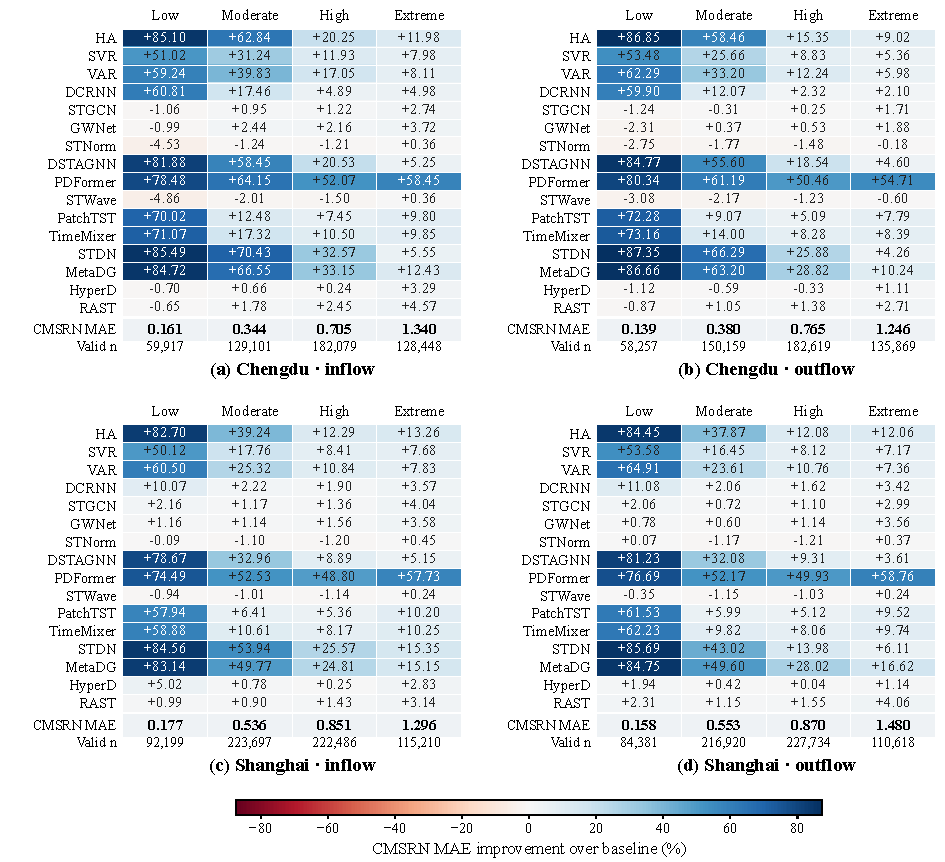
\includegraphics[width=\linewidth]{figures/scenarios/performance_h6_paper.pdf}
  \caption[常规模式偏离程度与H6预测性能]{\textbf{不同常规模式偏离程度下的H6预测性能。}四个面板对应成都和上海的流入、流出。单元格为\(100(\mathrm{MAE}_{m}-\mathrm{MAE}_{\mathrm{CMSRN}})/\mathrm{MAE}_{m}\)，正值（蓝色）表示CMSRN误差较低，负值（红色）表示相应基线误差较低。图中保留全部16种基线及统一色标；面板底部给出CMSRN的MAE和有效样本--网格数\(n\)。图内百分比保留两位小数。}
  \label{fig:scenario-performance}
\end{figure}

图~\ref{fig:scenario-performance}比较H6（提前30分钟）的分组表现。与总体结果表相比，情景分析另加入VAR、STNorm与STWave，构成16种基线的扩展比较。CMSRN在四项城市--通道任务中的MAE均随偏离等级升高而增大，但在Extreme组的相对排名更靠前：成都流入及上海两通道均排名第一，成都流出排名第三。前三项相对于最接近的基线STWave，MAE分别降低0.36\%、0.24\%和0.24\%；成都流出的MAE则比STWave高0.60\%。STNorm和STWave在多个较低偏离组中仍取得更低误差，表明CMSRN的相对竞争力具有情景和通道差异。

这一结果与本文关注局部流量偏离常规模式时的预测修正相呼应。与此同时，Extreme组的绝对误差仍较大，四项任务的MAE为Low组的7.32--9.38倍（补充图S1）。偏离等级还伴随流量规模变化，因此上述比较描述的是实际分组中的预测表现；其与残差通路的联系进一步由下述固定模型诊断考察。



\subsubsection{SERR在不同近期变化情景下的残差作用}\label{sec:scenario-serr}

在High与Extreme合并的高偏离子集中，以历史相邻标准化残差绝对差的均值描述近期变化强度，并按训练高偏离样本中该量的第75百分位数划分平缓变化（Slow）与快速变化（Rapid）两组。为考察已训练模型中各残差的实际作用，固定模型参数、门控和其余输出，分别从最终预测中扣除指定残差，计算
\begin{equation}
  \Delta\mathrm{MAE}_{e}
  =\mathrm{MAE}(\widehat Y-C_e)-\mathrm{MAE}(\widehat Y),
  \label{eq:scenario-residual-removal}
\end{equation}
其中\(C_e\)为实际加入预测的有符号修正量，包含门控、强度系数及逆标准化尺度。正值表示原残差降低了该组的平均MAE。该诊断与第\ref{sec:exp-ablation}节的独立重训练消融互为补充：前者度量锁定模型对既有修正的敏感性，后者比较重新训练后的修正通路配置。

图~\ref{fig:scenario-serr}中，两类专家在八个城市--通道--变化组上的16个移除差值均为正。自身残差在快速变化组的移除代价一致更大，为平缓组的1.61--2.82倍；例如，成都流入由0.0317增至0.0893，上海流入由0.0682增至0.1448。这说明，在当前高偏离样本中，节点自身演化修正在近期变化较快时对应更大的绝对MAE收益。时滞残差提供幅度较小的正向补充，其移除代价在成都的快速变化组增大，在上海则减小。两类角色呈现不同的情景响应，支持对自身动态与跨区域时滞信息分别组织修正证据。

\begin{figure}[!htbp]
  \centering
  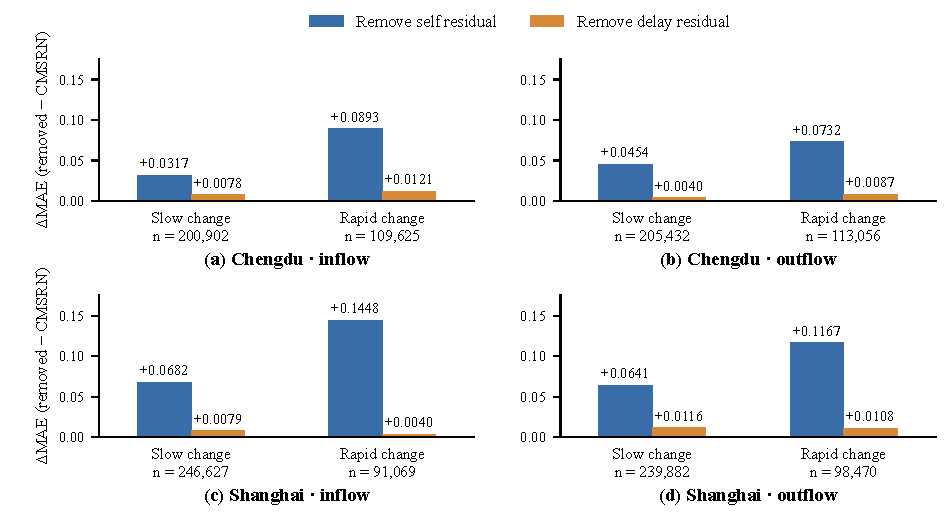
\includegraphics[width=0.92\linewidth]{figures/scenarios/serr_sensitivity_h6_paper.pdf}
  \caption[SERR在近期变化分组中的残差作用]{\textbf{高偏离情景下SERR的H6残差移除敏感性。}蓝柱和橙柱分别表示扣除自身残差与时滞残差后的\(\Delta\mathrm{MAE}\)，单位为原始5分钟流量计数；\(n\)为各组正目标样本--网格数。自身项扣除的是已加权的“自身预测减基础预测”修正。门控及其他残差保持不变，权重不重新归一化；两柱的MAE差值不具有可加性。}
  \label{fig:scenario-serr}
\end{figure}

\subsubsection{BCMS在不同背景差异与预测时距下的残差作用}\label{sec:scenario-bcms}

进一步在高偏离子集中，计算目标网格与各有效固定候选网格的历史平均标准化残差之差的绝对值，再对候选取均值，作为候选背景差异。使用训练高偏离样本的三分位阈值划分Low、Medium和High三组。该量由历史流量构造，是分析用的背景代理，并非BCMS内部学习到的低频表征。沿用式~\eqref{eq:scenario-residual-removal}，在H1--H12分别扣除完整BCMS修正，检查其作用随背景条件与预测时距的变化。

图~\ref{fig:scenario-bcms}显示，对每个城市、通道和预测步，低背景差异组的平均修正收益均高于中等组，中等组又高于高差异组。例如，上海流入在H6的三个\(\Delta\mathrm{MAE}\)依次为0.012448、0.008885和0.006301。144个背景组--预测步单元中有143个为正，唯一负值为成都流出高背景差异组H5的约\(-4.8\times10^{-6}\)。各组收益随预测步波动，未呈现随时距单调增加的规律。这些结果表明，BCMS的平均修正作用与候选背景条件有关，并在背景代理较接近的样本中更大。

将分析扩展至完整测试集后，各对应背景组--预测步的平均收益均高于高偏离子集，且仍保持低差异组高于中、高差异组的顺序（补充图S2）。例如，上海流入低背景差异组H6的\(\Delta\mathrm{MAE}\)由0.012448增至0.023927，表明BCMS的有效补充也覆盖其他交通状态。结合SERR的分组响应，自身演化修正在快速变化样本中具有更大的绝对MAE收益，而跨区域消息补充在背景代理较接近的样本中更有效。

\begin{figure}[!htbp]
  \centering
  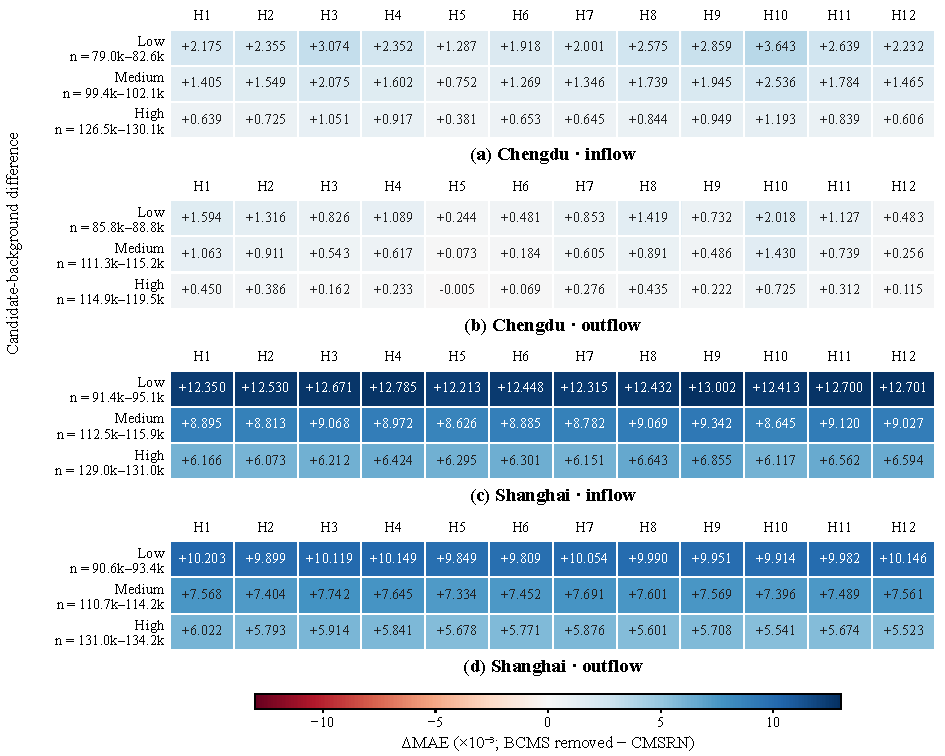
\includegraphics[width=0.92\linewidth]{figures/scenarios/bcms_sensitivity_horizons_paper.pdf}
  \caption[BCMS在背景差异与预测步分组中的残差作用]{\textbf{高偏离情景下BCMS的背景差异--预测步敏感性。}每格表示固定其余输出后扣除BCMS残差引起的MAE变化，数值按\(10^{-3}\)为单位显示，即图示值为\(1000\times\Delta\mathrm{MAE}\)。正值表示原修正降低组平均误差；H1--H12对应5--60分钟。背景组跨预测步保持固定，\(n\)的范围来自各步正目标位置数量的变化。该图为固定模型的输出移除诊断。}
  \label{fig:scenario-bcms}
\end{figure}

